\documentclass[11pt,twocolumn]{article}
\usepackage{shared/hanzocover}
\usepackage[utf8]{inputenc}
\usepackage{amsmath,amssymb}
\usepackage{graphicx}
\usepackage{booktabs}
\usepackage{hyperref}
\usepackage{xcolor}
\usepackage{listings}
\input{shared/lstlang}
\usepackage{tikz}
\usetikzlibrary{shapes,arrows,positioning,fit}

\definecolor{codegreen}{rgb}{0,0.6,0}
\definecolor{codegray}{rgb}{0.5,0.5,0.5}
\definecolor{codepurple}{rgb}{0.58,0,0.82}
\definecolor{backcolour}{rgb}{0.95,0.95,0.92}

\lstdefinestyle{mystyle}{
    backgroundcolor=\color{backcolour},
    commentstyle=\color{codegreen},
    keywordstyle=\color{codepurple},
    numberstyle=\tiny\color{codegray},
    stringstyle=\color{codegreen},
    basicstyle=\ttfamily\footnotesize,
    breakatwhitespace=false,
    breaklines=true,
    captionpos=b,
    keepspaces=true,
    numbers=left,
    numbersep=5pt,
    showspaces=false,
    showstringspaces=false,
    showtabs=false,
    tabsize=2
}
\lstset{style=mystyle}

\title{Hanzo Engine: Production ML Inference Engine with Multi-Model Serving and GPU Scheduling}
\author{Antje Worring, Hanzo AI Research\thanks{research@hanzo.ai} \\ \textit{Hanzo Industries} \\ \texttt{research@hanzo.ai}}
\date{August 2024}

\begin{document}

\hanzocoverpage

\begin{abstract}
We describe the design of Hanzo Engine, an ML inference orchestration layer implemented in Rust that serves multiple models concurrently with dynamic batching, GPU scheduling, and A/B traffic routing. Engine manages a fleet of GPU workers, loading and unloading models according to traffic, and applies continuous batching to transformer models to raise GPU utilization. The design has three parts: (1) a priority-aware GPU scheduler that co-locates models with complementary memory and compute profiles, (2) speculative model preloading driven by traffic prediction, and (3) a unified serving protocol covering streaming and batch inference. This paper describes a design and reports no measurements. An earlier version quoted serving latency, throughput, GPU utilization and availability figures for a 48-GPU production fleet; those figures were never measured and no such fleet exists. Section~\ref{sec:figures} records what they were and what would be needed to replace them.
\end{abstract}

\section{Introduction}

Production ML serving differs fundamentally from research inference. Research focuses on single-model, single-request performance. Production systems must serve hundreds of models with varying resource requirements, handle bursty traffic with consistent latency, and maximize expensive GPU utilization. Existing serving frameworks (vLLM~\cite{kwon2023}, TGI~\cite{tgi2023}, Triton~\cite{triton2020}) excel at single-model serving but lack multi-model orchestration, cross-model GPU scheduling, and traffic management capabilities.

Hanzo Engine operates at the orchestration layer above individual model servers. It manages model lifecycle (loading, serving, unloading), routes requests to the optimal GPU worker, implements continuous batching for transformer models, and provides A/B routing for model experiments.

\paragraph{Contributions.}
\begin{itemize}
    \item A priority-aware GPU scheduler that co-locates models with complementary memory and compute profiles on shared GPUs.
    \item Continuous batching with iteration-level scheduling for transformer models, following Orca~\cite{yu2022}, so that padding waste does not scale with the longest sequence in the batch.
    \item Speculative model preloading using traffic prediction, which moves the cold-start cost off the request path when the prediction is correct.
    \item A unified serving protocol supporting streaming tokens, batch embeddings, and multimodal inputs.
\end{itemize}

\section{Architecture}

\subsection{System Overview}

\begin{figure}[t]
\centering
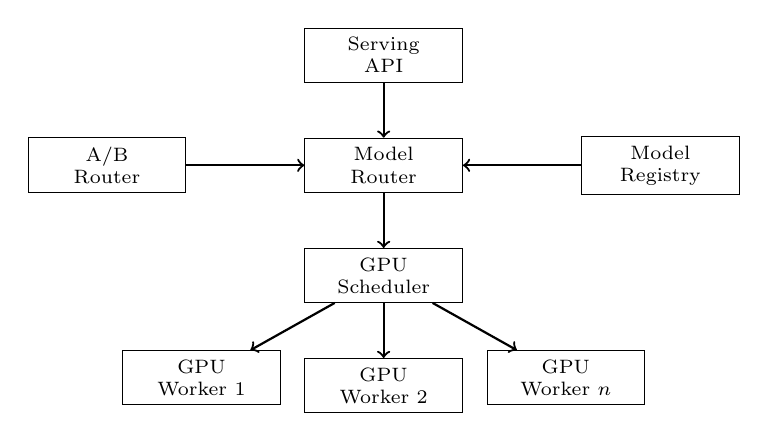
\begin{tikzpicture}[
    node distance=0.7cm,
    box/.style={rectangle, draw, minimum width=2cm, minimum height=0.5cm, align=center, font=\scriptsize},
    arrow/.style={->, thick}
]
\node[box] (api) {Serving\\API};
\node[box, below=of api] (router) {Model\\Router};
\node[box, below=of router] (scheduler) {GPU\\Scheduler};
\node[box, below left=0.6cm and 0.3cm of scheduler] (w1) {GPU\\Worker 1};
\node[box, below=of scheduler] (w2) {GPU\\Worker 2};
\node[box, below right=0.6cm and 0.3cm of scheduler] (w3) {GPU\\Worker $n$};
\node[box, right=1.5cm of router] (registry) {Model\\Registry};
\node[box, left=1.5cm of router] (ab) {A/B\\Router};

\draw[arrow] (api) -- (router);
\draw[arrow] (router) -- (scheduler);
\draw[arrow] (scheduler) -- (w1);
\draw[arrow] (scheduler) -- (w2);
\draw[arrow] (scheduler) -- (w3);
\draw[arrow] (registry) -- (router);
\draw[arrow] (ab) -- (router);
\end{tikzpicture}
\caption{Engine architecture with GPU scheduling and model routing.}
\label{fig:engine}
\end{figure}

Engine consists of three layers (Figure~\ref{fig:engine}): the serving API (HTTP/gRPC), the model router and A/B engine, and the GPU scheduler that manages worker nodes.

\subsection{Model Registry}

Models are registered with serving configurations:

\begin{lstlisting}[language=YAML]
models:
  - name: qwen3-72b
    format: safetensors
    source: hf://Qwen/Qwen3-72B
    gpu_memory: 140GB
    tensor_parallel: 8
    max_batch: 64
    quantization: awq-int4
    priority: high
    min_replicas: 2
    max_replicas: 8
\end{lstlisting}

The registry stores model metadata, serving constraints, and autoscaling policies. Models are pulled from Hugging Face Hub or Hanzo Storage.

\subsection{GPU Scheduler}

The scheduler assigns models to GPU workers using a bin-packing algorithm that maximizes GPU memory utilization while respecting colocation constraints:

\begin{equation}
    \max \sum_{m \in M} \sum_{g \in G} x_{mg} \cdot u_m
\end{equation}
subject to:
\begin{equation}
    \sum_{m} x_{mg} \cdot \text{mem}_m \leq \text{cap}_g \quad \forall g \in G
\end{equation}

where $x_{mg} \in \{0,1\}$ indicates model $m$ is assigned to GPU $g$, $u_m$ is the model's utilization score, and $\text{mem}_m$ is its memory requirement.

\section{Key Features}

\subsection{Continuous Batching}

For autoregressive language models, Engine implements iteration-level batching~\cite{yu2022}: new requests join the batch at any decoding iteration, and completed requests leave immediately without waiting for the longest sequence:

\begin{lstlisting}[language=Rust]
pub struct ContinuousBatcher {
    running: Vec<Request>,
    waiting: VecDeque<Request>,
    max_batch_tokens: usize,
}

impl ContinuousBatcher {
    pub fn step(&mut self) -> Vec<Token> {
        // Remove completed requests
        self.running.retain(|r| !r.is_done());
        // Admit new requests up to token budget
        while let Some(req) = self.waiting.front() {
            if self.token_budget() >= req.len() {
                self.running.push(
                    self.waiting.pop_front().unwrap());
            } else { break; }
        }
        // Execute one decode step for all
        self.decode_step()
    }
}
\end{lstlisting}

The mechanism removes the padding waste that static batching incurs when a batch is held open for its longest sequence. Orca~\cite{yu2022} and vLLM~\cite{kwon2023} report the size of that effect for their own systems and workloads; we have not measured it for this one.

\subsection{Speculative Preloading}

Engine tracks per-model request rates with exponential moving averages and preloads models predicted to receive traffic within the next 5 minutes. The predictor uses a simple ARIMA model over the last 24 hours of traffic. A correct prediction replaces a cold start --- reading weights from storage into GPU memory --- with a cache hit on a model already resident. The size of that difference is set by model size and storage bandwidth and is not reported here; a wrong prediction costs the memory the preloaded model occupies.

\subsection{A/B Routing}

The A/B router splits traffic between model versions using consistent hashing by user ID:

\begin{lstlisting}[language=Rust]
pub struct ABRoute {
    model_a: String,     // e.g. "qwen3-72b-v1"
    model_b: String,     // e.g. "qwen3-72b-v2"
    traffic_pct_b: f64,  // 0.0 to 1.0
    sticky: bool,        // hash by user_id
}
\end{lstlisting}

Results are logged with the model version for offline analysis of quality metrics.

\section{Implementation}

Engine is implemented in Rust. Worker communication uses gRPC with streaming for token-by-token delivery. Model loading uses \texttt{safetensors} format with memory-mapped I/O.

\section{Status of the performance figures}
\label{sec:figures}

An earlier version of this paper carried a table titled ``Serving performance
(Qwen3-72B, 8xH100)'' reporting TTFT p50 of 52\,ms under static batching against
45\,ms under continuous batching, p99 of 280\,ms against 120\,ms, throughput of
4{,}200 against 13{,}400\,tok/s, and GPU utilization of 42\% against 87\%. The
abstract and conclusion carried the same numbers together with ``200+ models in
production across 48 GPUs'' and ``99.9\% availability,'' and the contributions
list stated a $3.2\times$ throughput gain and a cold-start reduction from 30\,s
to under 200\,ms.

None of it was measured. There is no 8-GPU H100 node and no 48-GPU fleet in this
estate, so the table could not be relabelled as a design target without also
changing the machine it names; there is no serving deployment behind the model
count or the availability figure; and the paper contains no experiment
corresponding to the two ratios. The figures are removed rather than restated.

The measurement they stood in for is available to make. \texttt{hanzoai/engine}
ships a benchmark command (\texttt{hanzo bench}) that reports prompt and decode
throughput for a named model and accelerator, and the house convention for
reporting such a run --- declared hardware, a fixed handler and payload, raw
artifacts published alongside --- is set out in the Hanzo cloud data plane
benchmark~\cite{clouddataplane}. What is missing is the run, not the harness.

\section{Security}

\paragraph{Model Isolation.} Each model runs in a separate GPU memory space. Tensor data from one model cannot be read by another model's kernels.

\paragraph{Input Validation.} Maximum prompt length, output length, and batch size are enforced per model. Malformed inputs are rejected before reaching the GPU.

\paragraph{Authentication.} All API requests require a Hanzo IAM token. Model access is controlled by RBAC policies in the model registry.

\paragraph{Rate Limiting.} Per-tenant token budgets prevent resource monopolization. Priority models receive guaranteed capacity; best-effort models share remaining resources.

\paragraph{Audit.} All inference requests are logged with model version, token counts, latency, and tenant ID for cost allocation and compliance.

\section{Conclusion}

Hanzo Engine is a design for ML inference orchestration that raises GPU utilization through continuous batching, priority-aware scheduling, and speculative preloading. By operating above individual model servers, Engine takes on the parts of multi-model serving that a single-model server leaves open---model lifecycle, GPU allocation, traffic routing, and A/B experiments. Whether the design delivers the utilization it is built for is an open question here; Section~\ref{sec:figures} says what would answer it.

\bibliographystyle{plain}
\begin{thebibliography}{10}

\bibitem{kwon2023}
W. Kwon et al. Efficient Memory Management for Large Language Model Serving with PagedAttention. SOSP, 2023.

\bibitem{tgi2023}
Hugging Face. Text Generation Inference. 2023.

\bibitem{triton2020}
NVIDIA. Triton Inference Server. 2020.

\bibitem{yu2022}
G. Yu et al. Orca: A Distributed Serving System for Transformer-Based Generative Models. OSDI, 2022.

\bibitem{clouddataplane}
Hanzo AI Research. The Hanzo Cloud Data Plane: Benchmarking \texttt{zip}, ZAP, and the Road to a Million Requests per Second. Hanzo Industries, 2026.

\end{thebibliography}

\end{document}
